\documentclass{sigchi}

% Use this command to override the default ACM copyright statement (e.g. for preprints). 
% Consult the conference website for the camera-ready copyright statement.


% Arabic page numbers for submission. 
% Remove this line to eliminate page numbers for the camera ready copy
%\pagenumbering{arabic}



\usepackage{balance}  % to better equalize the last page
\usepackage{graphics} % for EPS, load graphicx instead
\usepackage{times}    % comment if you want LaTeX's default font
\usepackage{url}      % llt: nicely formatted URLs
\usepackage{graphicx}
\usepackage{caption}
\usepackage{subcaption}
\usepackage{array}

% llt: Define a global style for URLs, rather that the default one
\makeatletter
\def\url@leostyle{%
  \@ifundefined{selectfont}{\def\UrlFont{\sf}}{\def\UrlFont{\small\bf\ttfamily}}}
\makeatother
\urlstyle{leo}


% To make various LaTeX processors do the right thing with page size.
\def\pprw{8.5in}
\def\pprh{11in}
\special{papersize=\pprw,\pprh}
\setlength{\paperwidth}{\pprw}
\setlength{\paperheight}{\pprh}
\setlength{\pdfpagewidth}{\pprw}
\setlength{\pdfpageheight}{\pprh}

% Make sure hyperref comes last of your loaded packages, 
% to give it a fighting chance of not being over-written, 
% since its job is to redefine many LaTeX commands.
%\usepackage[pdftex]{hyperref}
%\hypersetup{
%pdftitle={L@S 2014 Work-in-Progress Format},
%pdfauthor={LaTeX},
%pdfkeywords={SIGCHI, proceedings, archival format},
%bookmarksnumbered,
%pdfstartview={FitH},
%colorlinks,
%citecolor=black,
%filecolor=black,
%linkcolor=black,
%urlcolor=black,
%breaklinks=true,
%}

% create a shortcut to typeset table headings
\newcommand\tabhead[1]{\small\textbf{#1}}

\begin{document}

\title{Exploring Classification}


\maketitle

\large

\section{Support Vector Machine}


We implemented the dual form of linear SVM's with slack variables in Python. To do so, we converted the input into a quadratic program, which we used \texttt{cvxopt.solvers.qp} to solve. Recall the general form of the quadratic program for the dual form of the SVM, which is given by

\normalsize
\begin{center}\begin{tabular}{r p{0.0in} l }
maximize && $ \displaystyle \sum_{i =1}^n \alpha_i - \frac{1}{2}\sum_{i = 1}^{n}\sum_{j = 1}^n \alpha_i\alpha_jy^{(i)}y^{(j)}(x^{(i)}\cdot x^{(j)}) $
\\ && \\
subject to && $ \displaystyle 0 \leq \alpha_i \leq C$ 
\\ && \\
&&		      $ \displaystyle \sum_{i = 1}^{n} \alpha_iy^{(i)} = 0$
\end{tabular}\end{center}

\large

We will demonstrate the formulation of this program in the matrix form required for \texttt{cvxopt.solvers.qp} on a simple example. Consider the dataset with positive examples $(1, 2)$ and $(2, 2)$ and negative examples $(0, 0)$ and $(-2, 3)$.
If we order the dataset according to the order presented here, then in matrix notation, the quadratic program above is given by

\normalsize
\begin{center}\begin{tabular}{r p{0.0in} l }
minimize &&\\
&&
$ \displaystyle \frac{1}{2}\alpha^T
\begin{bmatrix}
5 & 6 & 0 & -4\\
6 & 8 & 0 & -2\\
0 & 0 & 0 & 0\\
-4 & -2 & 0 & 13\\
\end{bmatrix}
\alpha +
\begin{bmatrix}
-1\\ -1\\ -1\\ -1\\
\end{bmatrix}^T
\alpha
 $
\\ && \\
subject to &&\\
&& $
\begin{bmatrix}
1 & 0 & 0 & 0\\
-1 & 0 & 0 & 0\\
0 & 1 & 0 & 0\\
0 & -1 & 0 & 0\\
0 & 0 & 1 & 0\\
0 & 0 & -1 & 0\\
0 & 0 & 0 & 1\\
0 & 0 & 0 & -1\\
\end{bmatrix}
\alpha
\leq
\begin{bmatrix}
C\\
0\\
C\\
0\\
C\\
0\\
C\\
0\\
\end{bmatrix}
$ 
\\ && \\
&&		      $ 
\begin{bmatrix}
1& 1& -1& -1\\
\end{bmatrix}
\alpha = \begin{bmatrix}0\end{bmatrix}
$
\end{tabular}\end{center}

\large
Solving this linear program for $\alpha$, we obtain the linear separator shown in Figure 1. For this small example, we can clearly see that this separator maximizes the margin.

\begin{figure}
\centering
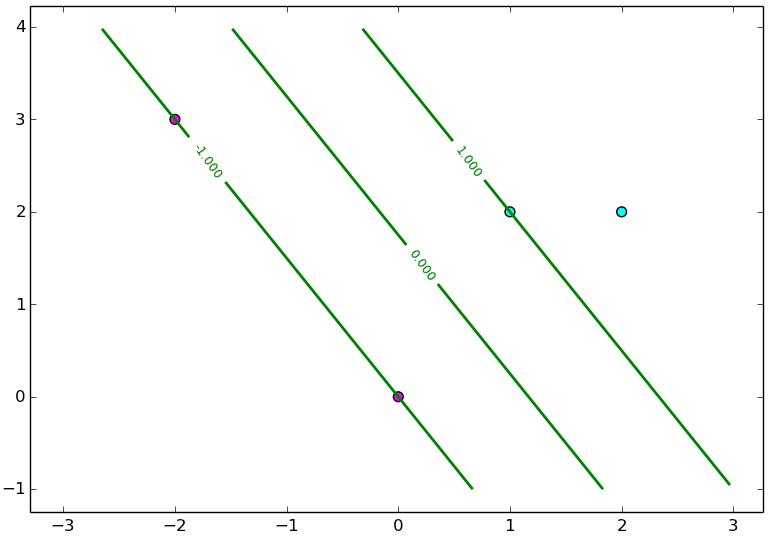
\includegraphics[width=2.25in]{plots/1-1.png}
\caption{test}
\end{figure}

\subsection{Applications}

Next, we try out our implementation on four different data sets, each consisting of 400 points. The first three data sets, which we will refer to as \texttt{stdev1}, \texttt{stdev2}, \texttt{stdev4}, consist of points where each of the negative and positive examples are generated from a Gaussian distribution with varying standard deviations (as suggested by the name). The final data set, \texttt{nonSep}, is a data set generated as to be impossible to separate with a linear separator.

For each of these data sets we will use a value of $C = 1$, and we will show the resulting boundary on both a training and validation set. We will also report the training and validation error rates. We begin with \texttt{stdev1}.

Figures 2(a) and 2(b) show the decision boundary formed by our algorithm on the training and validation data, respectively. As we can clearly see, both the training and validation data have an error rate of 0. This is not surprising given the very large gap between positive and negative samples.

Figure 2 also shows the results of repeating the process with \texttt{stdev2} and \texttt{stdev4}. For \texttt{stdev2}, the training error rate was 9.25\% and the validation error rate was 8.25\%. For \texttt{stdev4}, the training error rate was 26.5\% and validation error rate 23.5\%.

We can clearly see from the plots that \texttt{stdev2} and \texttt{stdev4} are not linearly separable (both in training and validation data), and thus we are not surprised by the increased error rates. It is interesting to note that the training data has higher error rates than the validation data in both cases. However, since both training data and validation data were drawn from Gaussian distributions, this is not terribly unlikely and does not surprise us.


\begin{figure*}[!ht]
\centering
\begin{tabular}{c c c}
\begin{subfigure}[b]{2.25in}
	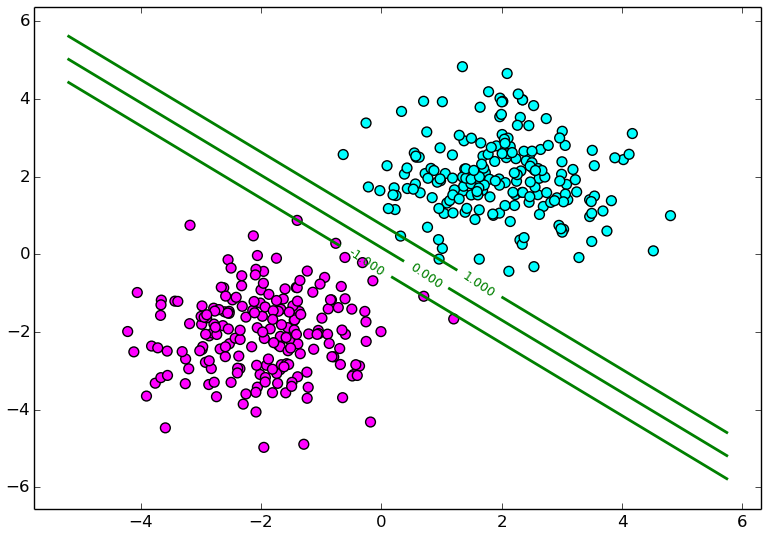
\includegraphics[width=2.25in]{plots/1-2/stdev1train.png}
	\caption{\texttt{stdev1} Training Data}
\end{subfigure} &

\begin{subfigure}[b]{2.25in}
	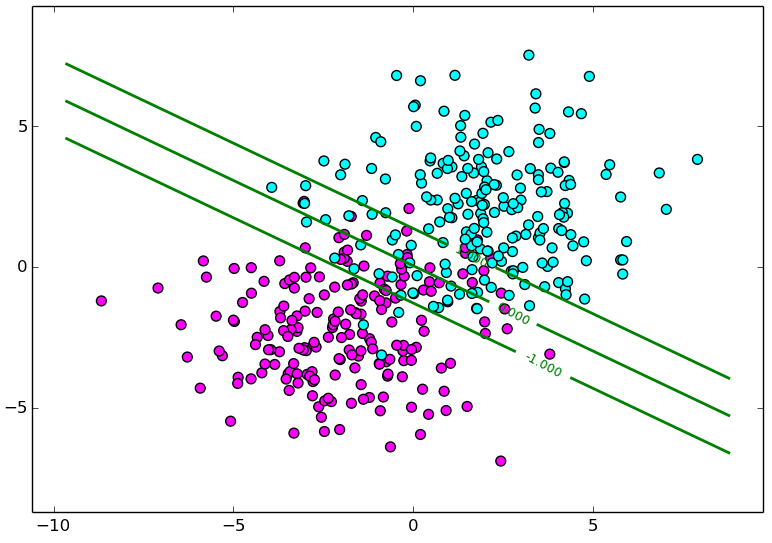
\includegraphics[width=2.25in]{plots/1-2/stdev2train.png}
	\caption{\texttt{stdev2} Training Data}
\end{subfigure} &

\begin{subfigure}[b]{2.25in}
	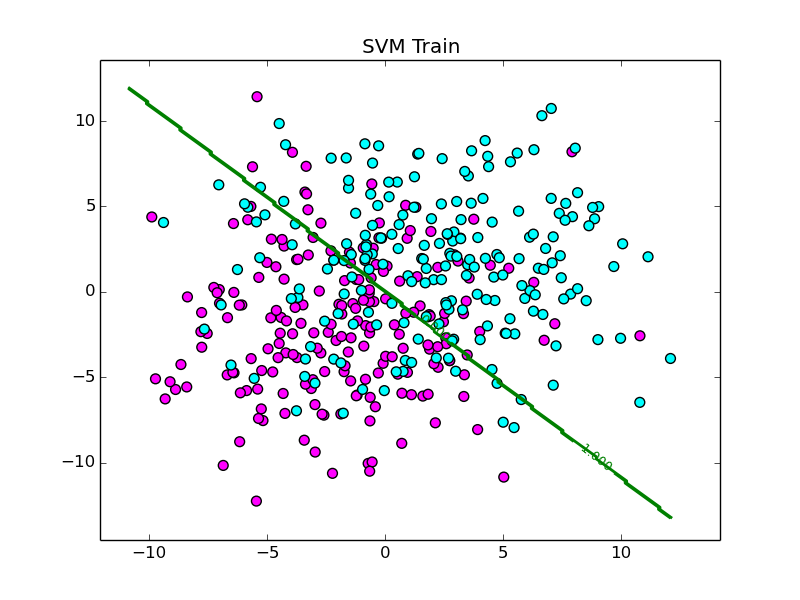
\includegraphics[width=2.25in]{plots/1-2/stdev4train.png}
	\caption{\texttt{stdev4} Training Data}
\end{subfigure} \\

\begin{subfigure}[b]{2.25in}
	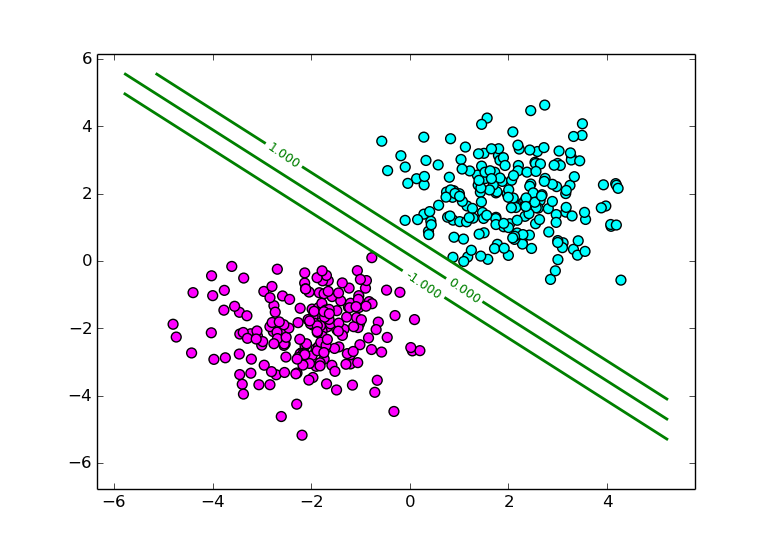
\includegraphics[width=2.25in]{plots/1-2/stdev1valid.png}
	\caption{\texttt{stdev1} Validation Data}
\end{subfigure} &

\begin{subfigure}[b]{2.25in}
	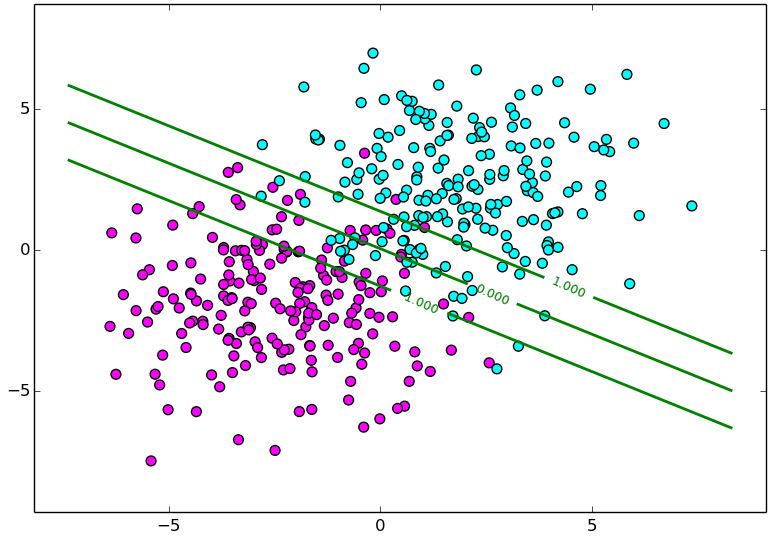
\includegraphics[width=2.25in]{plots/1-2/stdev2valid.png}
	\caption{\texttt{stdev2} Validation Data}
\end{subfigure} &

\begin{subfigure}[b]{2.25in}
	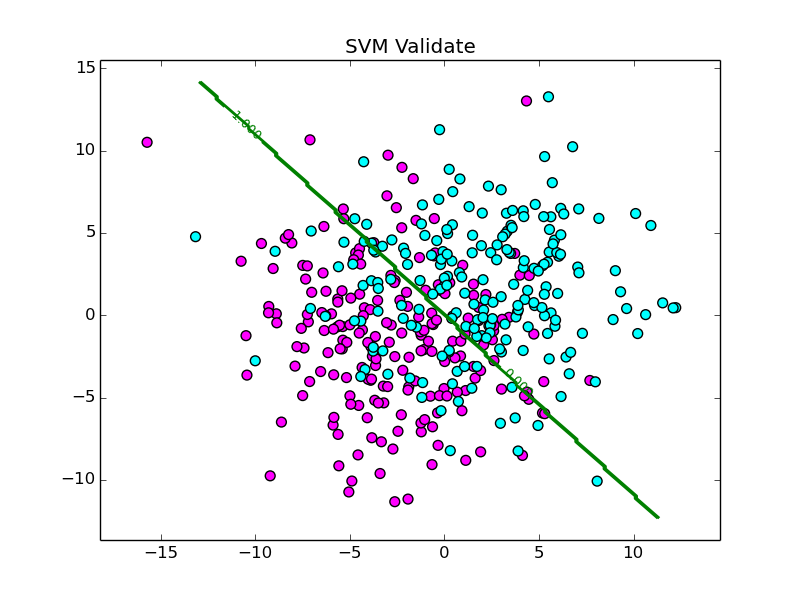
\includegraphics[width=2.25in]{plots/1-2/stdev4valid.png}
	\caption{\texttt{stdev4} Validation Data}
\end{subfigure} \\
\end{tabular}
\caption{test}
\end{figure*}

Next, we focus on \texttt{nonSep}. The resulting decision boundaries are shown in Figure 3. Clearly, this data is ill-fitted for classification via a linear separator.

\begin{figure}
\centering

\begin{subfigure}[b]{2.25in}
	\includegraphics[width = 2.25in]{plots/1-2/nonSep2train.png}
	\caption{\texttt{nonSep} Training Data}
\end{subfigure}

\begin{subfigure}[b]{2.25in}
	\includegraphics[width = 2.25in]{plots/1-2/nonSep2valid.png}
	\caption{\texttt{nonSep} Validation Data}
\end{subfigure}

\end{figure}

With a training error of 48.5\%, we can see that the separator is barely able to do a better job than randomly guessing how to classify each point. On the validation data, we see an error rate of 50.75\%. Because we have an error rate of over 50\%, we could have done a better job if we guessed the exact opposite of what our trained separator suggested. If we were not sure form the plot of the data that this data was not well suited to be classified using a linear separator, then the very high error rates convince us that this is in fact the case.

\subsection{Kernels}

Next, we extended our dual form SVM to operate with kernels. We experimented on our data using the Gaussian kernel, with a variety of values for $C$ and $\beta$. For each data set, we found the values of $C$ and $\beta$ which minimization the validation error rate. We repeated this experiment for the linear kernel, again using the validation error rate to tune $C$. The results are summarized in Figure 4.

\begin{figure*}
\centering
\renewcommand*{\arraystretch}{1.5}

\begin{tabular}{c c}
\begin{subfigure}[b]{3.5in}
\centering
	\begin{tabular}{| c | c | c | c | c |}
	\hline
	& \texttt{stdev1} & \texttt{stdev2} & \texttt{stdev4} & \texttt{nonSep}\\
	\hline
	$C$ & 1 & 0.01 & 0.01 & 10 \\
	\hline
	$\beta$ & 0.1 & 0.1 & 0.01 & 1 \\
	\hline
	SVs & 22 & 400 & 100 & 99 \\
	\hline
	Test Error & 0.25\% & 6\% & 21.75\% & 5\% \\
	\hline
	\end{tabular}
	\caption{Gaussian Kernel}
\end{subfigure}
&
\begin{subfigure}[b]{3.5in}
\centering
	\begin{tabular}{| c | c | c | c | c |}
	\hline
	& \texttt{stdev1} & \texttt{stdev2} & \texttt{stdev4} & \texttt{nonSep}\\
	\hline
	$C$ & 10 & 0.01 & 0.01 & 1 \\
	\hline
	SVs & 3 & 125 & 249 & 392 \\
	\hline
	Test Error & 0 & 7.25\% & 22\% & 49.5\%\\
	\hline
	\end{tabular}
	\caption{Linear Kernel}
\end{subfigure}
\end{tabular}

\caption{test}
\end{figure*}

To get an idea for how the classifier works using a Gaussian kernel, Figure xx shows the resulting classifier for \texttt{stdev1} and \texttt{nonSep}. We can clearly see that the classifier is no longer linear. In addition, we can see that on this allows for it to handle the \texttt{nonSep} data in a way which the linear separator could not.

\begin{figure}
\centering

\begin{subfigure}[b]{2.25in}
	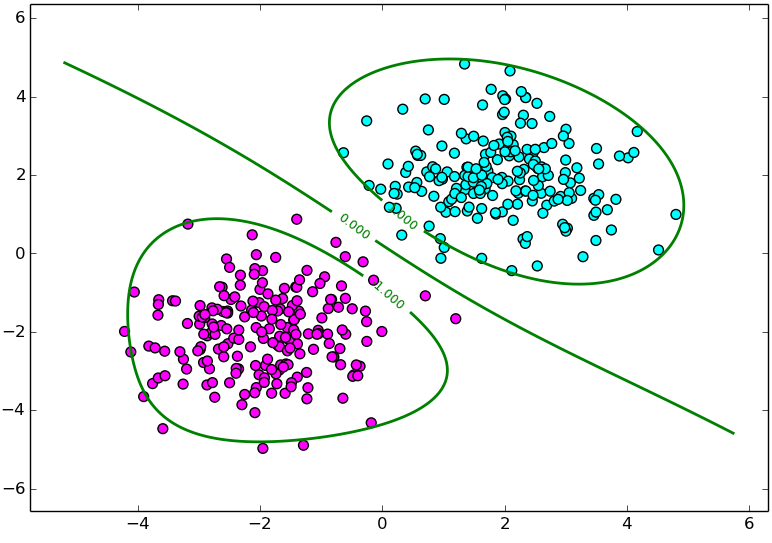
\includegraphics[width = 2.25in]{plots/1-3/stdev1opttrain.png}
	\caption{$C = 0.01$}
\end{subfigure}

\begin{subfigure}[b]{2.25in}
	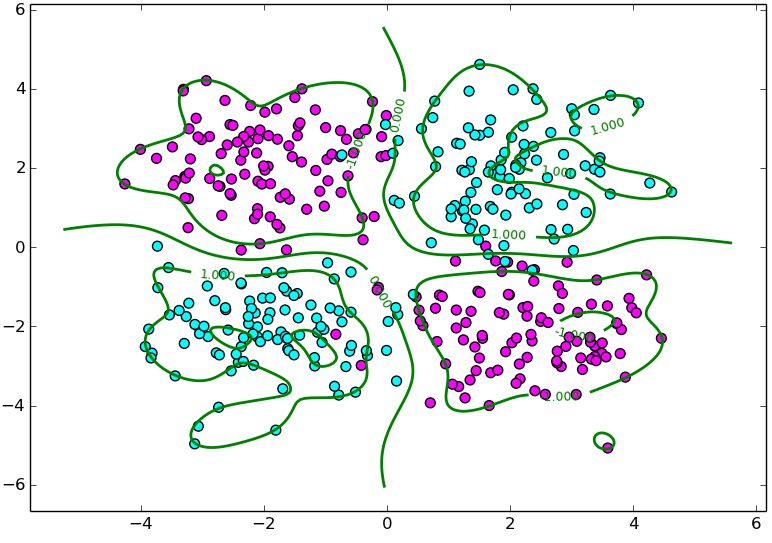
\includegraphics[width = 2.25in]{plots/1-3/caseychart.png}
	\caption{$C = 100$}
\end{subfigure}

\end{figure}

For \texttt{stdev1}, \texttt{tdev2}, and \texttt{stdev4}, we can see that the test error rates resulting from both the Gaussian and linear kernels are very similar. From looking at the data sets, it seems that a linear separator is the most appropriate choice for the data. Thus, even when we apply a Gaussian separator, which allows a lot more flexibility, we still find that the linear separator performs roughly equally well.

For \texttt{nonSep}, we see a much different story. The data is clearly not linearly separable. Thus, we are hardly able to achieve an error rate below 50\% with the linear separator. However, when we apply the Gaussian separator, we are able to achieve an error rate of only 5\%. Thus, the added flexibility of the Gaussian kernel allows us to use the same techniques to separate data which is not linearly separable.

Figure 4 also shows the number of support vectors that the optimal parameters returned. We note that these numbers may be slightly misleading. Because \texttt{cvxopt.solvers.qp} never actually drove $\alpha$ values completely to zero, we had to choose a threshold such that we considered only $\alpha$ values above the threshold to be support vectors. For all of our experiments, we chose a value of $10^{-5}$. From observation, this value seemed to most accurately represent a cutoff between $\alpha$ values which were significant and those which seemed as if they should be considered zero.

It is interesting to note that for all data sets other than \texttt{stdev1} (which was completely linearly separable and thus did not actually require any slack), the number of support vectors in the optimal solution was very high. It is possible that our threshold for deciding support vectors just did not do an adequate job of deciding which points should be considered support vectors. However, experimenting with the threshold value and the parameters of the solver did not yield any better results. We also note that for \texttt{stdev2} and \texttt{stdev4}, the value of $C$ is very small. In the next section, we will discuss the effect that the value of $C$ has on the number of support vectors.

\subsection{Analyzing C}

Next, performed experiments to analyze the effects of varying $C$. Our goal is to examine how the value of $C$ affects the value of the geometric margin and the number of support vectors chosen using the linear kernel. Note that the notion of geometric margin does not make sense for the Gaussian kernel. However, we note that the dependence of the number of support vectors on $C$ was similar in the Gaussian kernel as in the linear kernel. We will show our results for data sets \texttt{stdev1} and \texttt{stdev2}. The results for the other two data sets are similar, so we do not display them here.

For each of \texttt{stdev1} and \texttt{stdev2}, we used $C$ in the set $\{0.01, 0.1, 1, 10, 100\}$, and computed the geometric margin and total number of support vectors. As a general trend, both the geometric margin and the number of support vectors decreased as we increased $C$. % Increasing C means less slack

We can see this in Figure xx, which shows the separator defined by $C = 0.01$ and $C = 100$ for \texttt{stdev1}. We can clearly see that the increased value of $C$ results in a margin smaller margin, and consequently must fewer vectors are support vectors.

\begin{figure}
\centering

\begin{subfigure}[b]{2.25in}
	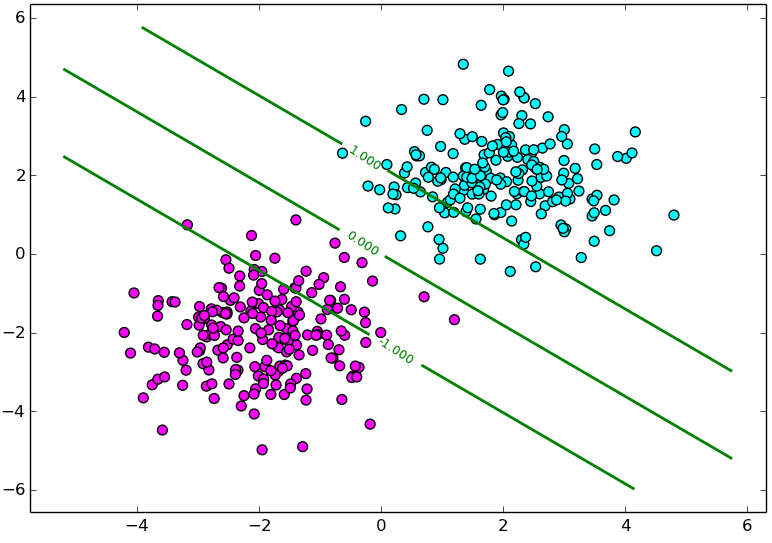
\includegraphics[width = 2.25in]{plots/varyingC/001.png}
	\caption{$C = 0.01$}
\end{subfigure}

\begin{subfigure}[b]{2.25in}
	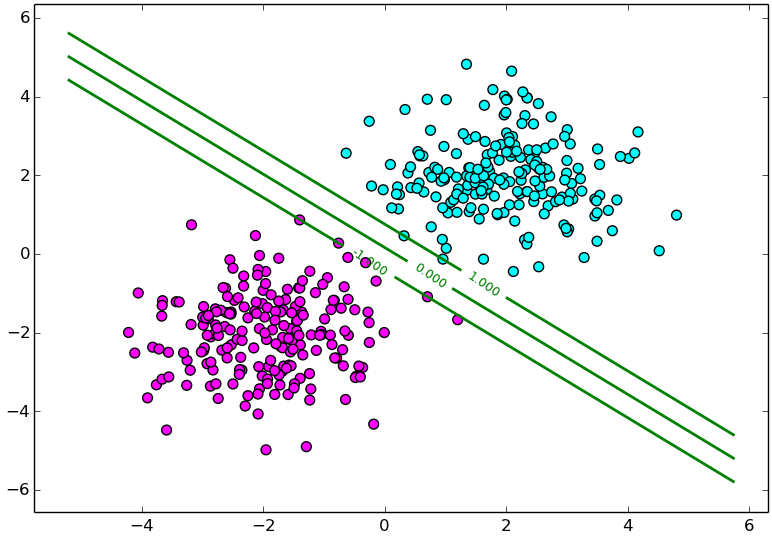
\includegraphics[width = 2.25in]{plots/varyingC/100.png}
	\caption{$C = 100$}
\end{subfigure}

\end{figure}

Figure xx shows geometric margin and number of support vectors plotted as a function of $C$. Note that the $x$ axis is shown on a log scale for convenience. We can see that both the geometric margin and number of support vectors seem to decrease to a point and then level off. This is because as we increase $C$, we decrease the amount of slack that we allow. As $C$ approaches infinity, we approach the situation where we do not allow any slack.

\begin{figure}
\centering

\begin{subfigure}[b]{2.25in}
	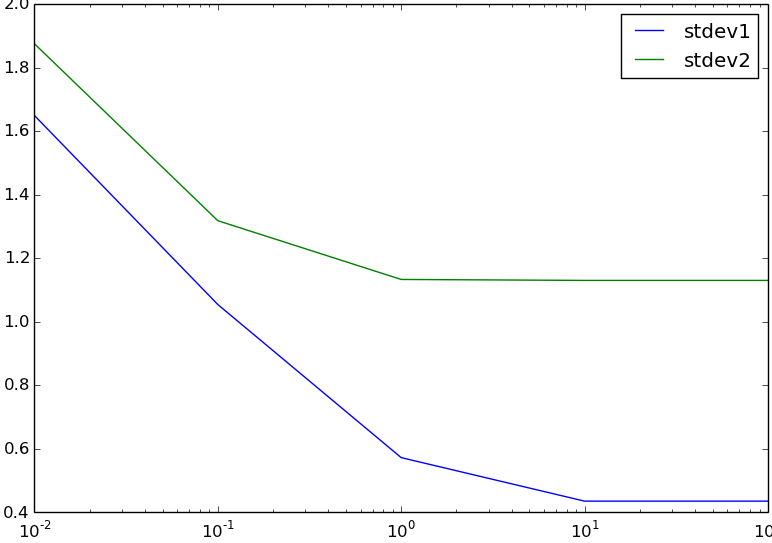
\includegraphics[width = 2.25in]{plots/1-3/margin.png}
	\caption{Geometric Margin}
\end{subfigure}

\begin{subfigure}[b]{2.25in}
	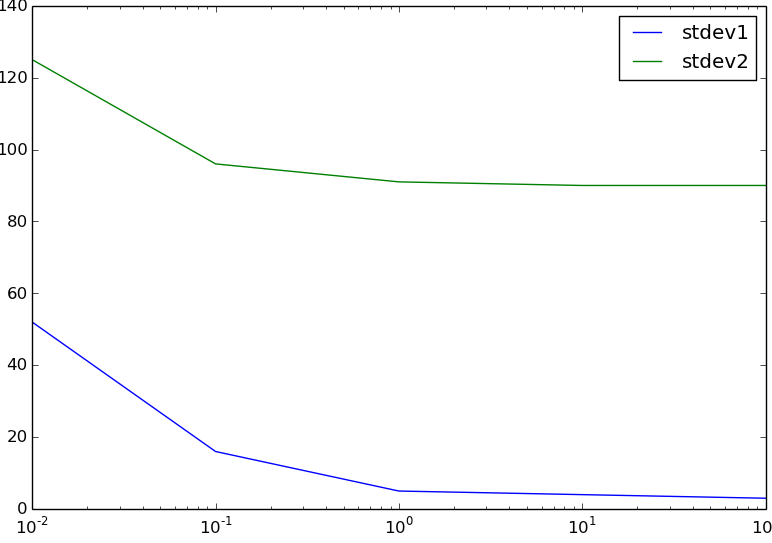
\includegraphics[width = 2.25in]{plots/1-3/support_vectors.png}
	\caption{Number of Support Vectors}
\end{subfigure}

\end{figure}

We know that a support vector machine aims to maximize the size of the margin. Thus, a seemingly reasonable idea would be to use $C$ to maximize the value of the margin on the training data. However, from the trends we see above, this seems that it would just result in the choice of an arbitrarily small value for $C$, which we would have no reason to expect to perform well on the validation or test data.

A more reasonable choice is to choose $C$ based on the validation data. An option would be to maximize the size of the margin on the validation data. However, from Figure xx we can see that increasing the margin can just lead to more vectors being classified as support vectors, which does not actually improve our classification accuracy. The option which tended to give better overall performance was to choose $C$ to minimize the validation error rate.

\section{Logistic Regression}

\section{Multi-Class Classification}

In the previous sections, we dealt with data that needed to be classified as positive or negative. In this section, we will discuss data that needs to be classified as one of $\{1, \hdots, k\}$. In particular, we will deal with the problem of predicting the forest cover type (of which there are 7) of a region based on a 54-dimension feature vector, a problem based on the Kaggle challenge. We will apply both support vector machine and logistic regression techniques.

We were given 15,120 data points, which we randomly split into three sets of size 5,040 to serve as the training, validation, and testing data.

\subsection{Support Vector Machines}

We implemented multi-class support vector machines using the one-versus-the-rest approach. We tested the Kaggle data using both the linear and Gaussian kernel, and found that we were able to achieve a much higher success rate with the linear kernel. We attributed this difference to overfitting of the training data with the Gaussian kernel.

Moving forward with the linear kernel, we begin training the model on the training set and using the validation error rate to tune the value of $C$. Because solving the quadratic program with the support vector machine takes prohibitive amounts of time when run on our training set of 5,040 points, we used a smaller subset of the training and validation sets to tune $C$ (1000 points each).

We found that the best value of $C$ was $C = 1$. Figure xx shows the resulting validation errors for various values of $C$. With this set, we were able to achieve a success rate of xx\% on the test data (when trained on the subsets of training and validation data).

\begin{figure}
\renewcommand*{\arraystretch}{1.5}
\begin{tabular}{| c | p{.25in} | p{.25in} | p{.25in} | p{.25in} | p{.25in} |}
\hline
$C$ & \centering 0.01&  \centering 0.1 & \centering 1 & \centering 10 & 100 \\
\hline
Validation Error & & & & & \\
\hline
\end{tabular}
\caption{Validation Error for various values of $C$}
\end{figure}

Due to time and space constraints, we did not explore any other approaches for handing the fact that our algorithm was not able to efficiently train on the entire training set. One possible option would have been to have performed the computation on a more powerful machines (such as Amazon Web Services). With 8GB of RAM, the machine on which we did the training was completely overtaken by performing the training on the full training set. Another option would have been to abandon our implementation of the SVM and use another implementation which supported Sequential Minimal Optimization, in order to provide an approximate solution in a much more manageable timeframe.

Once we settled on a value of $C$, we performed training on all 5,040 training points. The computation managed to terminate after a few hours. With this model, we were able to achieve a success rate of XX\% on the test data. We note that the original data contained equally many points in each class, so this is far better than the 14\% success rate that we would expect from a model which did not actually have any information about the data set.

\subsection{Logistic Regression}

\subsection{Discussion}

Here we should probably talk about how SVM's can achieve slightly higher accuracy, but take much longer and can only train on much smaller data sets. Perhaps the logistic regression would perform better if it had the opportunity to train on more data?






\section{Logistic Regression}

\subsection{Theory}

The kernelized form of the logistic regression objective can be derived as follows. We know that the negative log likelihood function, which we want to mininize, can be expressed as follows:

$$NLL(w) = \sum_{i=0}^N \log(1+e^{-y^{(i)}(x^{(i)}\cdot w + w_0)}) $$

where for a data point i, $y^{(i)}$ represents what class it belongs to and $x^{(i)$ represents what its feature vector was. $w$ and $w_0$ together make up the weights, supplied by the algorithm and used to classify the points.  The algorithm will tend to classify a point as having a positive label if $x^{(i)} \cdot w + w_0$ is positive and as having a negative label if the $x^{(i)} \cdot w + w_0$ is negative. More precisely, the algorithm assigns a probability of $\frac{1}{1+e^{-W^T x}}$ to the point's correct classification being positive, and a probability of $1 - \frac{1}{1+e^{-W^T x}}$ to the point's correct classification being negative. In light of this, the above formula for a posteriori negative log likelihood makes sense; it is therefore our goal as algorithmicists to minimize this quantity as efficiently as possible. \\

The natural method to use to minimize the negative log likelihood is by the method of gradient descent. This will require repeated calls to the formula defined above, for an indefinite period of time before the value converges or our algorithm gives up. Each such call takes a certain amount of time: given that the outer sum loops over $N$ different elements (where $N$ is the number of data points), and each call to the function requires us to evaluate $x^{(i)} \cdot w$, the dot product of two $d$-dimensional vectors (where $d$ is the dimensionality of the feature vectors), every call to $NLL(w)$ as defined above will take $\Theta(Nd)$ time to compute, assuming basic arithmetic operations are constant-time. \\

This is efficient assuming $N = \Omega(d)$. However, in the case where $d >> N$, it is possible to do much better than this by making a clever assumption. We may assume that $W = X^T \alpha$. Here, $W$ is our $d+1$-dimensional vector of weights that helps us determine how we will ultimately classify points ($W$ includes $w$ and $w_0$, $X$ is a $N \times d+1$ matrix that contains of record of every data point and the features it contains, preceded by a 1 (to allow for the offset term $w_0$); the $i^{\textrm{th}}$ row of $X$ is $\{1 x^{(i)}\}$. Finally, $\alpha$ is some new $N$-dimensional vector for us to consider, which roughly corresponds to how important each of the data points is to our classification. The core idea is to transform the above formula from being a formula over inputs $W$ (a $d$-dimensional vector) to a formula over inputs $\alpha$ (an $N$-dimensional vector). \\ 

We derive this transformation as follows:

$$NLL(w) = \sum_{i=0}^N \log(1+e^{-y^{(i)}(x^{(i)}\cdot w + w_0)}) $$
$$NLL(w) = \sum_{i=0}^N \log(1+e^{-y{(i)}(XW)^{(i)}})$$
In the equation above, $(XW)^{(i)}$ denotes the $i^{\textrm{th}}$ element of the vector $XW$. \\

Next, we make use of the assumption $W = X^T\alpha$.
$$NLL(\alpha) = \sum_{i=0}^N \log(1+e^{-y^{(i)}(XX^T\alpha)^{(i)}})$$
$$NLL(\alpha) = \sum_{i=0}^N \log(1+e^{-y{(i)}((XX^T)^{(i)} \cdot \alpha})$$

We now have a new formula, with a new vector on which we can do gradient descent. Moreover, the dimensionality of the new vector is different from that of the old vector; $\alpha$ is an $N$-dimensional vector, in contrast to $W$, which was a $d$-dimensional vector. \\

How long does it take to compute the formula above? Well, naively, one might expect that we need to iterate over the sum $N$ times, and for each iteration of the sum, we need to compute the matrix product $XX^T$, which takes $\Theta(N^2d)$ time (the runtime of multiplying an $N \times d$ matrix with a $d \times N$ matrix). Then, we need to compute the dot product of $(XX^T)^{(i)}$, an $N$-dimensional vector, with $\alpha$, another $N$-dimensional vector, which would take $\Theta(N)$ time. Thus, at first glance, it appears that our new formula takes $\Theta(N^3 d)$ time to compute; not an improvement! \\

However, this naive calculation is missing an important insight: the matrix $XX^T$ can be precomputed. Because it is independent of $\alpha$, there's no reason for us to compute it at every step of the gradient descent. Instead, we will compute it once, at the start of the algorithm, and then every at every step of the gradient descent, we will not need to recompute it. With that consideration taken into account, each step of the gradient descent will now take $\Theta(N^2)$ time. This \emph{is} quite an improvement over the old runtime of $\Theta(Nd)$, assuming $N << d$. \\

We call this new form of the equation above the \emph{kernelized} form of the equation. It allows us to efficiently find a weight vector $W$ even when the feature space is very large, by doing gradient descent on the $\alpha$ vectors, and then computing $W$ at the end by using the fact that $X^T\alpha = W$. \\

Moreover, this method can be used to substitute in an arbitrary kernel matrix in place of $XX^T$. Thus, this general method supports the use of any kernel one chooses, simplying by plugging in a precomputed kernel matrix and running gradient descent. \\

One potential issue with this method is that it will have a tendency to assign a non-zero value to every $\alpha$, since in logistic regression, every point has some effect on the location of the classifier, albeit often small. This is not ideal; for many applications, it is convenient to have an $\alpha$ that is very sparse, in order to make computations involving $\alpha$ cheaper and in order to make the situation easier to describe and understand. \\

For this reason, we introduced L1 regularization on the $\alpha$ values; in other words, we introduced an additional penalty of $\lambda ||\alpha||_1$ on the alpha vectors, in addition to the penalty corresponding to the negative log likelihood. Our overall penalty $P(\alpha)$ for a given vector $\alpha$ was: \\

$$P(\alpha) = NLL(\alpha) + L1(\alpha)$$
$$P(\alpha) = \sum_{i=0}^N \log(1+e^{-y{(i)}((XX^T)^{(i)} \cdot \alpha}) + \lambda||\alpha||_1$$

In order to introduce the L1 regularization without adversely affecting the performance of the gradient descent function (functions that are not smooth can disrupt gradient descent functions) we used the approximately-correct function 

$$L1(\alpha) \approx \lambda \sum_i \sqrt{||\alpha_i||^2 + \epsilon}$$

for some sufficiently small $\epsilon << \lambda$. 

\subsection{Experiment}

As a test of our methods, we used them on the 2D data sets. In these tests, we used the fmin_bfgs function for our gradient descent, available online.

 Our methods yielded results that seemed to strongly imply an underlying mechanism that made sense.  

Our results, with $\lambda = 0$, are shown below:

\begin{figure}
\centering

\begin{subfigure}[b]{2.25in}
	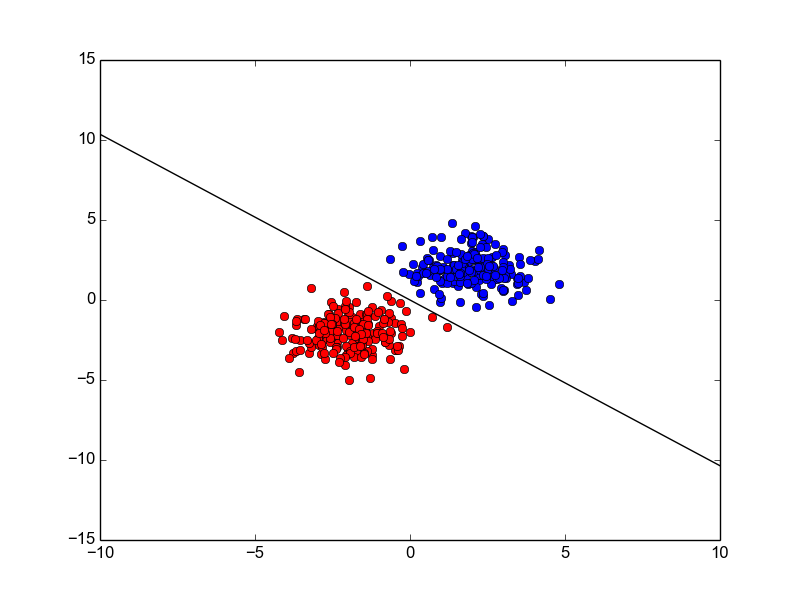
\includegraphics[width = 2.25in]{plots/stdev1_train_plot.png}
	\caption{Our separator, shown on the training data, for data drawn from low-variance Gaussians.}
\end{subfigure}

\begin{subfigure}[b]{2.25in}
	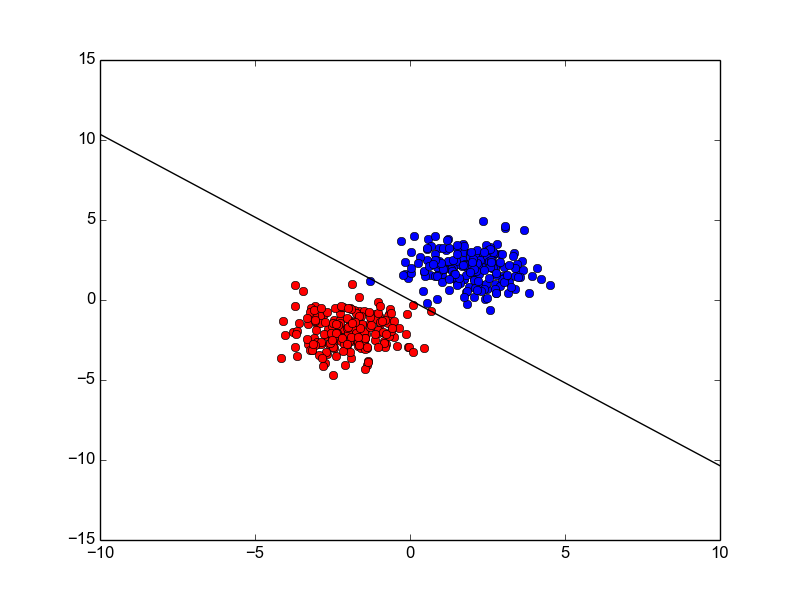
\includegraphics[width = 2.25in]{plots/stdev1_test_plot.png}
	\caption{Our separator, shown on the test data, for data drawn from low-variance Gaussians}
\end{subfigure}

\end{figure}

\begin{figure}
\centering

\begin{subfigure}[b]{2.25in}
	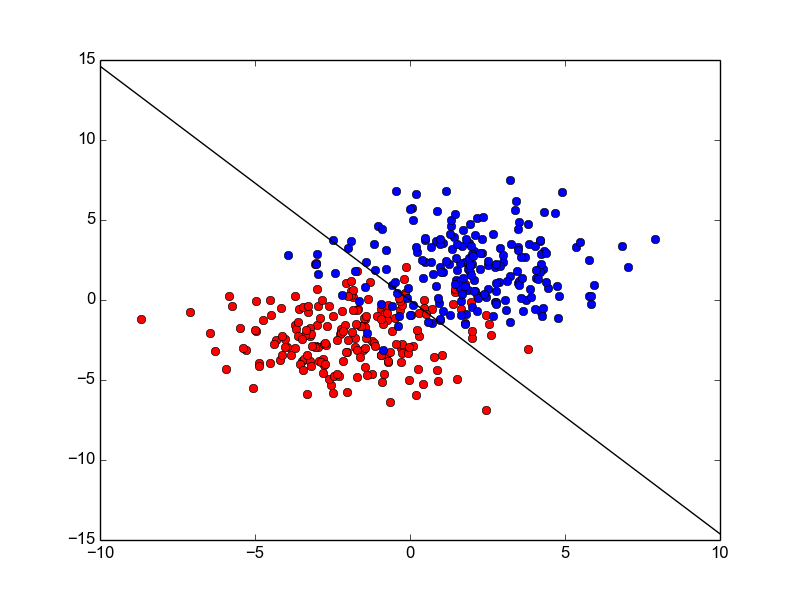
\includegraphics[width = 2.25in]{plots/stdev2_train_plot.png}
	\caption{Our separator, shown on the training data, for data drawn from mid-variance Gaussians.}
\end{subfigure}

\begin{subfigure}[b]{2.25in}
	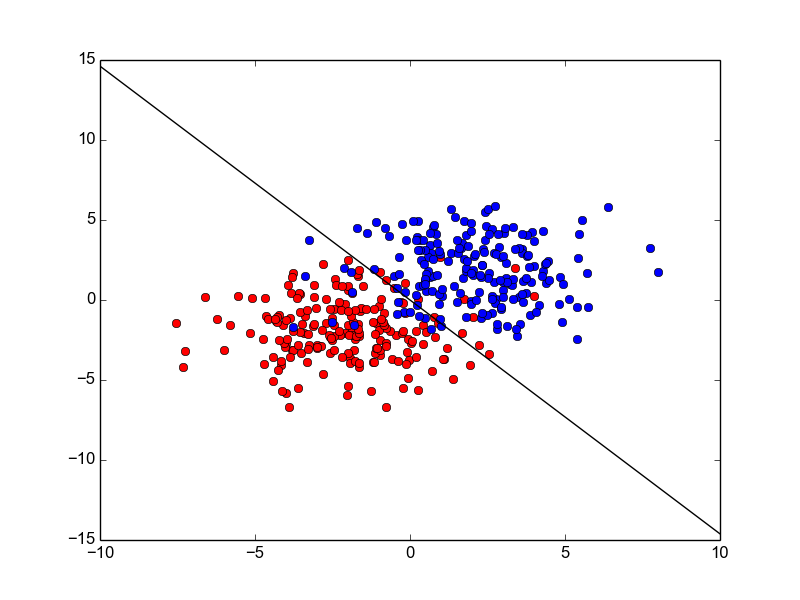
\includegraphics[width = 2.25in]{plots/stdev2_test_plot.png}
	\caption{Our separator, shown on the test data, for data drawn from mid-variance Gaussians}
\end{subfigure}

\end{figure}

\begin{figure}
\centering

\begin{subfigure}[b]{2.25in}
	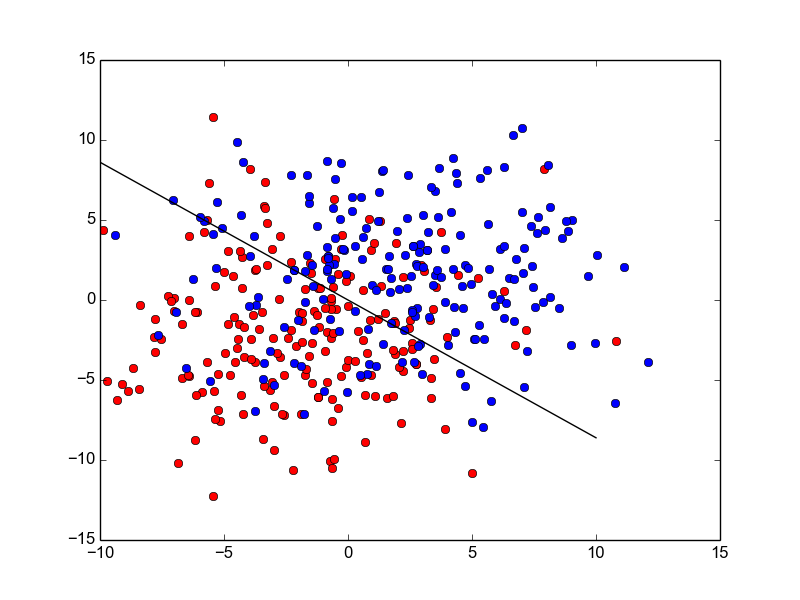
\includegraphics[width = 2.25in]{plots/stdev4_train_plot.png}
	\caption{Our separator, shown on the training data, for data drawn from high-variance Gaussians.}
\end{subfigure}

\begin{subfigure}[b]{2.25in}
	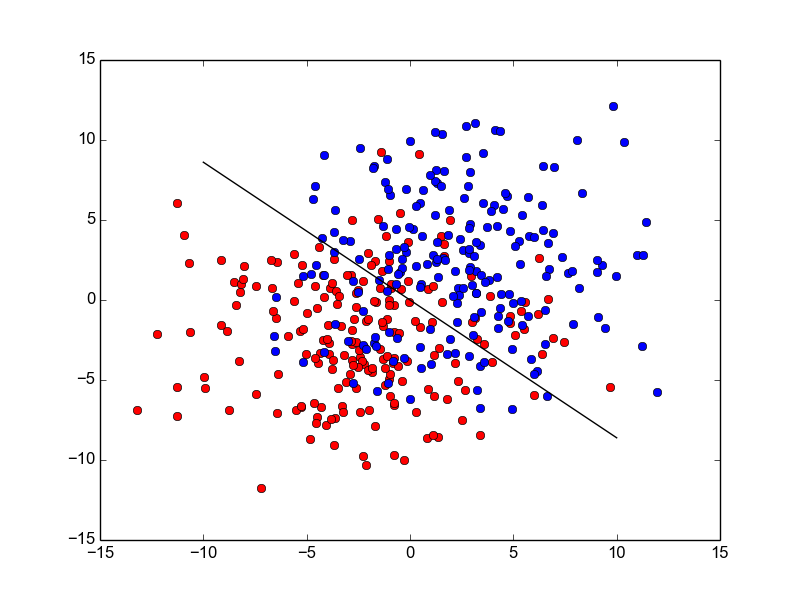
\includegraphics[width = 2.25in]{plots/stdev4_test_plot.png}
	\caption{Our separator, shown on the test data, for data drawn from high-variance Gaussians}
\end{subfigure}

\end{figure}

\begin{figure}
\centering

\begin{subfigure}[b]{2.25in}
	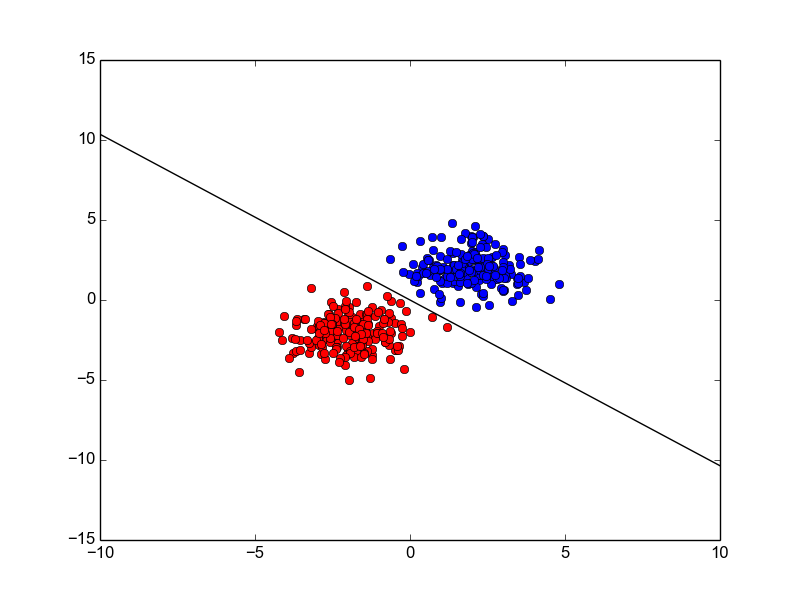
\includegraphics[width = 2.25in]{plots/stdev1_train_plot.png}
	\caption{Our separator, shown on the training data, for data drawn from low-variance Gaussians.}
\end{subfigure}

\begin{subfigure}[b]{2.25in}
	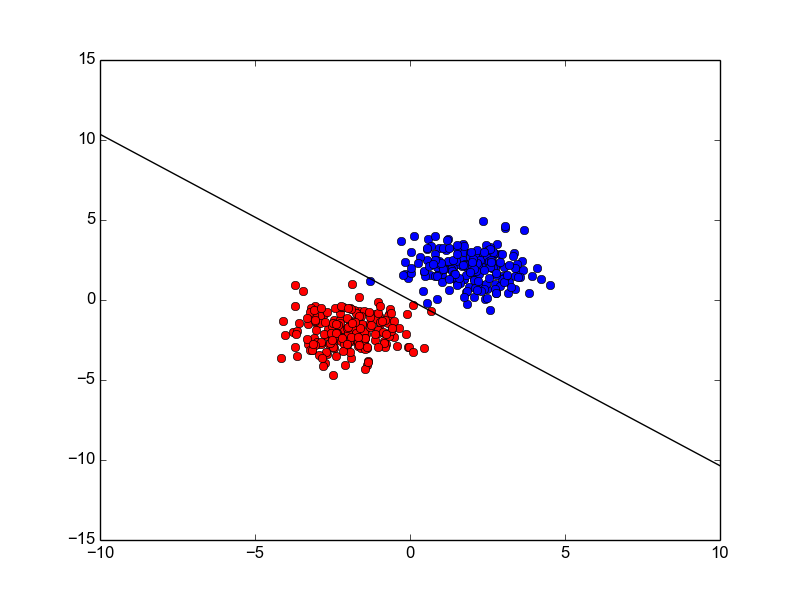
\includegraphics[width = 2.25in]{plots/stdev1_test_plot.png}
	\caption{Our separator, shown on the test data, for data drawn from low-variance Gaussians}
\end{subfigure}

\end{figure}

\end{document}